\documentclass[../main.tex]{subfiles}
\begin{document}
\tikzstyle{container} = [draw, rectangle, inner sep=0.3cm, dashed, minimum height=3.5cm]
In the last 50 years car have transitioned from being composed only by mechanical parts to being completely stacked with electronics. The complexity of vehicles arises every year and the industry continuously raise the bar on the state of the art. The transitions to electro-mobility, the ADAS systems have done all but slowing down the development. The more a topic is market relevant, the higher the competition between companies, the faster the development in that field is going to be. The automakers are always ready to exploit or create new needs in order to adapt and attract customers. Automotive pulse of innovation and the "German Silicon Valley" is the place a engineer want to be to fell part of this complex, but for sure perfectly oiled, machine.   
\begin{figure}
\centering
\begin{minipage}{.5\textwidth}
  \centering
  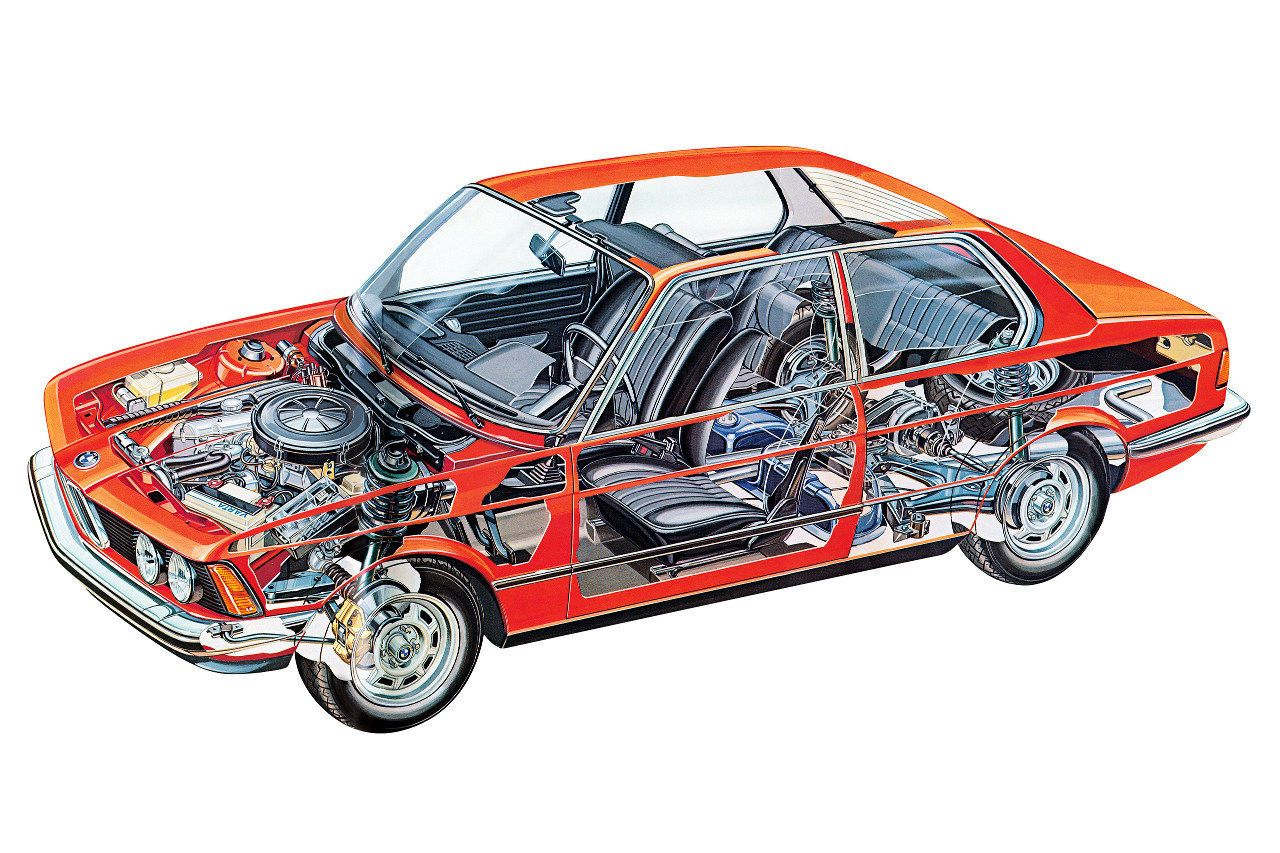
\includegraphics[width=\linewidth]{images_folder/4a56e1d50b56da42a10e29d451cf2b93.jpg}
  \caption{BMW 320 Coupe - 1975}
  \label{fig:test1}
\end{minipage}%
\begin{minipage}{.5\textwidth}
  \centering
  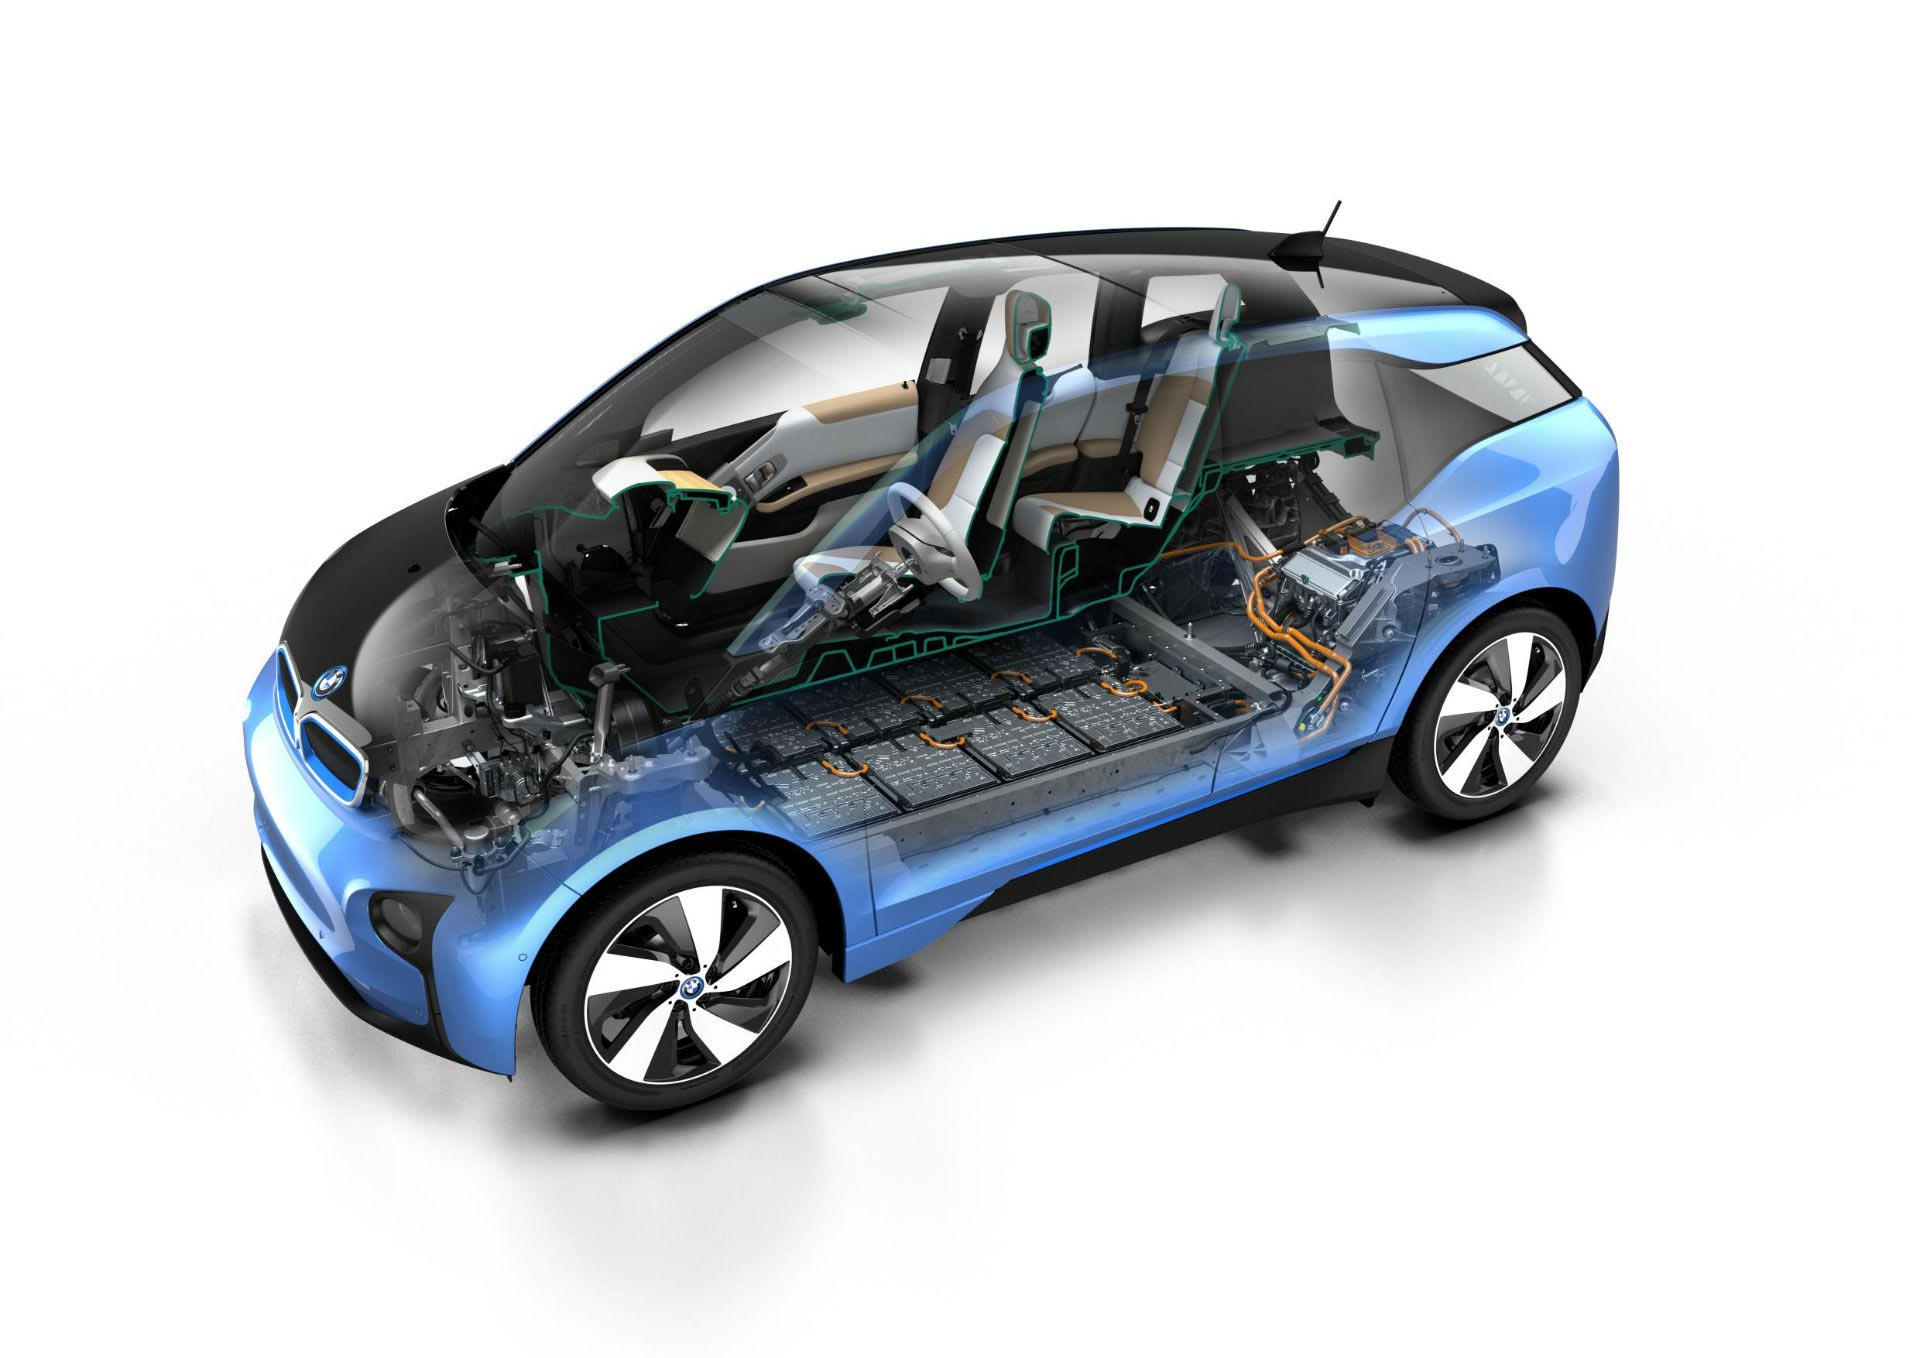
\includegraphics[width=\linewidth]{images_folder/BMW_i3.jpg}
  \caption{BMW I3 - 2015}
  \label{fig:test2}
\end{minipage}
\end{figure}

\section{Block Schema of a car}
The complexity of system car can be easily simplified by block schemes. Block schemes are going to be a recursive topic during the thesis, thanks to the outside view that they allow to have on complex topics. 
    \begin{figure}[ht]
        \begin{center}
  \begin{tikzpicture}[auto, node distance=3cm,>=latex', scale=0.7,transform shape]
            \node [input1, name=input] {};
            \node [sum1, right=of input] (sum) {};
            \node [block1, right=of sum] (controller) {$Vehicle \;System$};
            \node [output, right=of controller] (output) {};
            \draw [draw,->] (input) -- node {$User\; inputs$} (sum);
            \draw [->] (sum) -- node {} (controller);
            \draw [->] (controller) -- node [name=y] {$(speed,\; position..)$}(output);
            \draw [->] (y) -- ++ (0,-3) -| node [pos=0.99] {$-$} (sum);
            \end{tikzpicture}
        \end{center}
    \caption{Block Scheme of a car}
    \end{figure}
The input to the \textit{vehicle system} can be an array of driver commands, such as the steering, throttle position and all the settings that control the car. The output of the system is not only the movement of the car, but also more driver specific feeling such as the drive comfort or just the temperature in the vehicle. The \textit{vehicle system} can be further inspected, exposing two other block that are basic in the vehicle, the one responsible for the electronics and the one responsible for the mechanics. 
     \begin{figure}[ht]
        \begin{center}
  \begin{tikzpicture}[auto, node distance=3cm,>=latex', scale=0.7,transform shape]
            \node [input1, name=input] {};
            \node [sum1, right=of input] (sum) {};
            \node [sum, right=of sum] (sum_A) {};
            \node [block, right=of sum_A] (controller) {$Electronics$};
            \node [block, right=of controller] (mechanics) {$Mechanics$};
            \node [output1, right=of mechanics] (output) {};
            \draw [draw,->] (input) -- node {$User\; inputs$} (sum);
            \draw [->] (sum) -- node {} (sum_A);
            \draw [->] (sum_A) -- node {} (controller);
            \draw [->] (controller) -- node {} (mechanics);
            \draw [->] (mechanics) -- node [name=y] {$(speed,\; position..)$}(output);
            \draw [->] (mechanics) -- ++ (0,-2) -| node [pos=0.99] {$-$} (sum_A);
            \draw [->] (y) -- ++ (0,-4) -| node [pos=0.99] {$-$} (sum);
            % \node [container,fit=(controller) (mechanics) (sum_A)] (container) {};
            \end{tikzpicture}
        \end{center}
        \caption{Sub block division}
    \end{figure}       
These two blocks are strictly interconnected. The electronics drive the mechanics which output is given back as a feedback to correct the response. Continuing with the analogies, the system vehicle can be considered as a complex version of an embedded system where electronics drive mechanics following a logic described in lines of code.
Every mechanical component in cars has probably some electronic hardware related to it which is controlled by one of the many ECUs (Electronic control Units) in the vehicle. The increasing presence of embedded devices in the vehicle required a rapid increase in the software in order to control it. The yearly increase in lines of code for cars reported in \ref{fig:yearlyincreas} is a statement supporting of the importance of software. 
\begin{figure}[H]
    \centering
    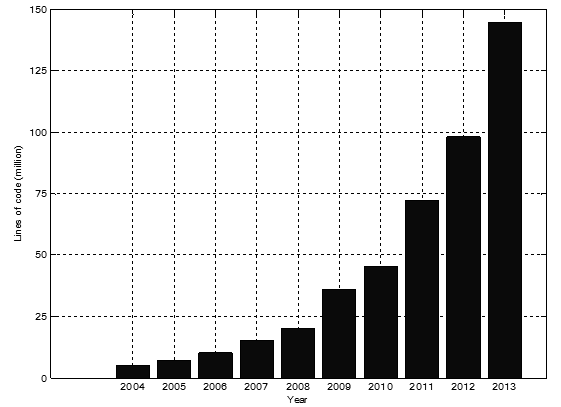
\includegraphics[width=0.6\linewidth]{images_folder/Yearly-increase-in-automotive-software-complexity-shown-by-million-lines-of-code-of-1-ConvertImage.png}
    \caption{Yearly increase in automotive software complexity}
    \label{fig:yearlyincreas}
\end{figure}
The fact that line of code are increasing mean a increasing complexity in the development process, which translate to requirement of a higher scalability and portability during the whole development process. The main in the thesis is going to focus on how this software is developed, generated and adapted to different ECUs. 
\section{ECU software}
The development of Software for ECUs is an extremely complex task, a single ECU can control up to a 1000 functions, and the number can be also higher for the control of complex parts, such as the motor.
Consider the following example. The function related to the control of the windshield wipers. In a scheme block manner we can see that the first indication comes from the driver, which activates the switch for the control of the windshield wipers. The signal travel to the ECU where it´s analyzed based on a logic stated in code lines. the output of the logic is then sent to the actuators specific board, which in this case actuates a motor that control the windshield wipers.\\
\begin{figure}[H]
    \centering
    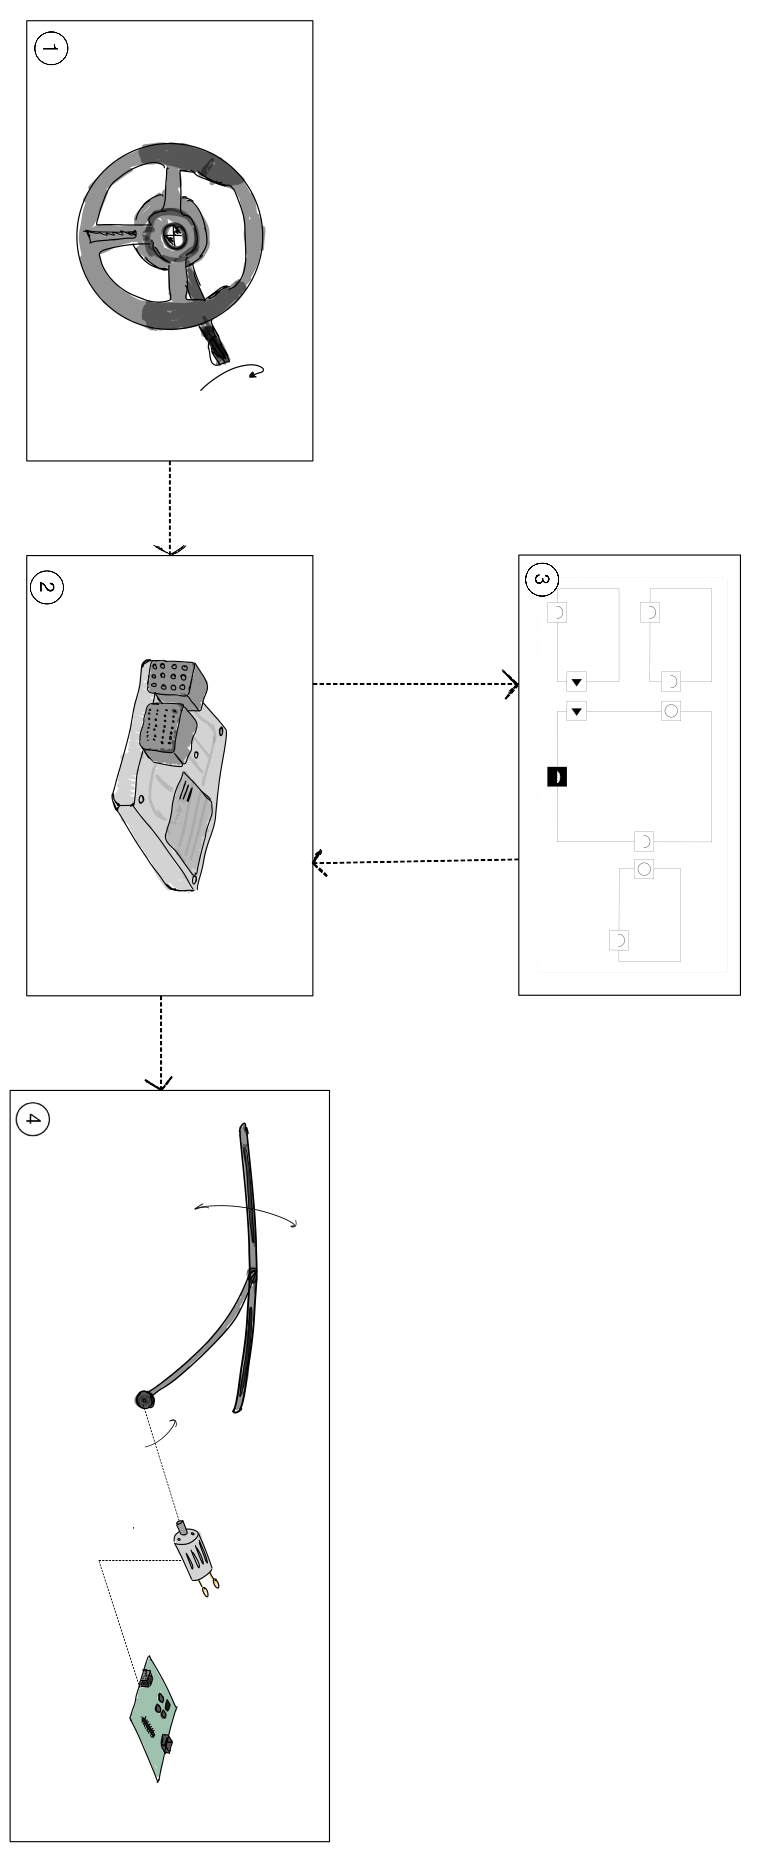
\includegraphics[width=0.45\linewidth, angle = 90]{images_folder/windshieldwipersfunction.jpeg}
    \caption{Windshield wipers function}
    \label{fig:WWFunct}
\end{figure}
The task seems like a basic one, consider now thousand of task sending contemporaneously information to the ECU. The ECU, indeed,  elaborates thousand of input signals every second and output the control at the same rate. In order to make everything work there are major problem that need to be considered:
\begin{itemize}
    \item Task prioritization, every function need to be assigned a priority, in order to be executed from the ECU. Windshield wiping need to have a lower priority than airbag deployment. Every task arriving to the ECU need to be prioritize following a logic. 
    \item Task scheduling, task need to be scheduled to meet deadlines, since ECUs are Real Time System, one of the requirements is that the system not only provide an output but provide and output under certain time constraints. 
    \item Access to shared resources, multiple task may require the ECU to read the same sensor or to act on the same actuator, or more deeply access the same memory location. The ECU need to control the access to these resources to avoid error but also to avoid saturation, which can lead to restarts and failure.  
    \item Failure handling, the ECU need to have the capabilities to avoid failure and to continue operating in case of failing hardware/software.
    \item Task predictability, task need to be designed to be predictable in their functionality, this allow to extend the predictability to the ensemble of tasks, and therefor predict the behaviour of the entire ECU. 
\end{itemize}
The work of developing not only the logic behind tasks, but also the logic that control how task need to work in the system is one of the complex parts in the ECU design. 
\subsection{ECU software design for tasks}
The design of software for a single function, such as the one reported in \ref{fig:AUTCA} can be separated in two parts:
\begin{itemize}
    \item Task software, software related to the control of the actual task. 
    \item integration software, part of the software responsible for the integration with other tasks, usage of shared resources and all the other real time requirements. 
\end{itemize}
The software is developed using a model based design approach. By using the Matlab Simulink tool the developer create the logic for the single function using blocks. The Simulink models contains the following macro information:
\begin{itemize}
    \item Logic information, related to the control of input and output signals.
    \item integration information, related to where the functions integrates. 
    \item Use of resources, like shared memory or communication interfaces like the CAN bus
    \item IO capabilities, if a function require the read of particular sensors in order to compute the logic. 
\end{itemize}
All those information need to be packed in a readable format for the ECU hardware. The process of compilation of the code, integration with the system and IO functionalities need is taken care by a dedicated software. 
At BMW this dedicated software has been internally developed in python. The software takes as input all the functions and gives as an output the artifacts useful to be flashed in the ECU. 
The ECU can´t read a Matlab block, so the first step is to create executable code. 
\subsection{Build Process}
\label{subsection:Build process}
The build software has the function of compiling, linking, integrating, testing and validating the different functions developed for a certain ECUs. \\
The build process perform the following tasks:
\begin{itemize}
    \item Compilation and linking, the build compile the single function, generation executable code. 
    \item Architectural check, the build, after having build all the function, integrates them. For example multiple function can require the output of another one. There is the need to check if this output is available and therefore the different function can integrate together.
    \item Quality checks, every software unit need to be checked based on Misra rules and other coding standards for developing safety-critical systems as the ECU.
    \item Unit Testing and static code analysis, that analyze the software before this is compiled and deployed in the ECU
    \item Documentation, generate documentation for every software components. 
    \item Artifacts archiving, the output artifacts need to be published in a repository. 
\end{itemize}
\begin{figure}[H]
    \centering
    \begin{tikzpicture}[mindmap, grow cyclic, every node/.style=concept, concept color=gray!10, text width=]
    \node{Build}
    	child { node {Compilation}}
    	child { node {Architectural Check}}
    	child { node {Quality Checks}}
    	child { node {Documentation}}
    	child { node {Unit Testing}}
    	child { node {Linking}}
    	child { node {Artifacts Archiving}};
\end{tikzpicture}
    \caption{Caption}
    \label{fig:my_label}
\end{figure}
The output of the build run is what BMW provide to the actual ECU makers, such as Bosch and Vitesco, they add their software part, closely related to the hardware that they develop. The composition of this package is flashed on the ECU, on which is further tested via HIL, SIL practices.\\
After testing the ECUs are installed on the car.
\section{Statement of Problem}
The build system analysis underline a complex set of data that is generated throughout the process. Referring to \ref{subsection:Build process} it´s easy to grasp the complexity of the process. It´s important also to highlight the fact that each of the steps of the process are supervised by different people. This makes the output information hard to grasp for the developer that is not in charge of the specific part of the process. Even if the Agile like practices makes cooperation strong in between the team that develop and maintain the build software and also with the teams that develop function, a central view on all the artifacts is missing.\\
The need for a centralized overview that can allow the developers to surf through different information regarding the whole developer step is missing. A way to efficiently give a overview of the process is the use of a dashboard, that not only would allow for a graphical visualization but also for an easy way to look for data. In order to be useful inside a fast phased project the dashboard need to have the following characteristics:
\begin{itemize}
    \item Usability, the dashboard need to be easy to use and interactive, in the term that need to provide a rapid way to look for data from different sources. 
    \item Accessibility, all the team need to have access to the visualization
    \item Real time data, the dashboard need to be backed by always updating data. This allow to have a real time picture of the full ECU software build. This is required because as multiple developer make changes on different parts of the process, if the dashboard is not able to quickly give a feedback of these changes than it´s not useful for the developer as a source of feedback. 
\end{itemize}
\section{Thesis Motivation}
\section{Thesis Goals}
\section{Contribution to the thesis}
\cleardoublepage
\end{document}